\chapter{پیچیدگی ارتباطی}\label{chapter1}


\par
مدل پیچیدگی ارتباطی در ابتدا در سال 1970 توسط Yao معرفی شد و هدف آن این است که یک مساله‌ را به صورت توزیع‌شده\footnote{Distributed} حل کند. منظور از حل به صورت توزیع‌شده آن است که افراد مختلف، با در دست داشتن آرگومان‌های مختلف از یک مساله مشخص، با همکاری هم به حل مساله بپردازند. مهم‌ترین نکته در این مدل این است که افراد دخیل در مخابره، قدرت محاسباتی نامحدود دارند و تنها فاکتور مورد بررسی، مقدار پیام‌های رد و بدل شده میان آ‌ن‌هاست.
 مطالب این فصل با اقتباس از 
 \cite{ 
 		nissan09,
 		lee09,
 		tim15,
 		toni14,
 		sherstov18
 		}
 تهیه شده است.


\section{تعریف}

یک پروتکل قطعی پیچیدگی ارتباطی، پروتکلی مانند $\pi$ است که در هر مرحله، یکی از دو طرف مخابره، پیامی یک بیتی به دیگری می‌فرستد. آلیس (A) ورودی $x \in X$ را در اختیار دارد و باب (B) ورودی $y \in Y$. هدف این پروتکل این خواهد بود که این دو نفر با هم خروجی $z \in Z$ را محاسبه کنند، به صورتی که:
\[val(\pi(x, y)) = f(x, y) \quad \forall x \in X, y \in Y\]
که در آن $f$ یک تابع دانسته توسط دو طرف است.
\par

\textbf{  درخت پروتکل: }
معادل با تعریف بالا، می‌توان یک درخت پروتکل باینری در نظر گرفت که رئوسش تصمیم‌ها (بیت‌های ارسال شده) توسط بازیکنان و برگ‌هایش خروجی‌ها هستند:

\begin{itemize}
    \item هر یک از رئوس غیر برگ درخت یا به آلیس تعلق دارند و یا باب.
    \item هر راس داخلی $v$ که به آلیس تعلق دارد، معادل با تابع $A_v: X \rightarrow \{0,1\}$ است که بیت فرستاده‌شده توسط آلیس را وقتی به این راس برسد، با توجه به ورودی وی تعیین می‌کند.
    \item هر راس داخلی $v$ که به باب تعلق دارد، معادل با تابع $B_v: X \rightarrow \{0,1\}$ است که بیت فرستاده‌شده توسط باب را وقتی به این راس برسد، با توجه به ورودی وی تعیین می‌کند.
    \item هر برگ این درخت ($l$) یک مقدار $val(l) \in Z$ دارد.
\end{itemize}

هر جفت ورودی $x \in X, y \in Y$ در مدل قطعی، یک مسیر یکتا از ریشه تا یک برگ را تعیین می‌کنند. هزینه یک پروتکل، معادل با عمق درخت (بلندترین مسیر از ریشه تا برگ) است که با $D(f)$ مشخص می‌شود.

\par
از آنجایی که آلیس می‌تواند کل رشته‌اش را برای باب بفرستد و این حداکثر مکالمه مورد نیاز بین دو طرف است، برای یک تابع $f: \{0,1\}^n \times \{0,1\}^n \rightarrow \{0, 1\}$، $D(f) \leq n + 1 $ است.

\par

نکته قابل توجه این است که همواره می‌توان یک درخت پروتکل را متوازن کرد. به عبارت دیگر، یک درخت پروتکل با $N$تا برگ با درخت پروتکل دیگری با عمق $O(log\ N)$ معادل است. به بیان دیگر، عمق درخت به عنوان یک شاخص برای اندازه‌گیری پیچیدگی ارتباطی، به جز یک ضریب ثابت، با لگاریتم تعداد برگ‌های درخت معادل است.


\section{تکنیک‌های کمینه‌یابی}
زمانی که صحبت از پیچیدگی به میان می‌آید، لازم است که مشخص شود یک مساله مشخص حداقل به چه مقدار زمان یا حافظه برای رسیدن به جواب نیاز دارد. در مورد مسائل پیچیدگی ارتباطی، پیچیدگی مورد نظر همان تعداد بیت مخابره شده بین افراد مکالمه است. منظور از کمینه\footnote{lower-bound} برای این نوع پیچیدگی، کمترین تعداد بیت‌هایی است که بین دو نفر جابه‌جا خواهد شد تا پاسخ مساله $p$ با سایز ورودی $n$
بر دو طرف آشکار باشد. در مورد پیچیدگی ارتباطی و کمینه‌هایش در ابتدای راه قرار داریم ولی در حال حاضر تکنیک‌های سومندی برای مشخص کردن کمینه یک مساله تعریف و استفاده شده‌اند که ابتدا مفاهیم اولیه پیش‌نیاز را مطرح خواهیم کرد و در ادامه به بررسی هر یک از ابزارها می‌پردازیم.

\subsection{ماتریس مشخصه}
با توجه به تابع از قبل مشخص $f: X \times Y \rightarrow \{0, 1\}$، ماتریس مشخصه\footnote{Characteristic Matrix} تابع $f$ به صورت زیر است:
\begin{center}

    $M_{f} = [f(x,y)]_{x \in X, y \in Y}$

\end{center}
اگر $X=\{x_{1}, x_{2},...,x_{m}\}$ و $Y=\{y_{1}, y_{2},...,y_{n}\}$، شکل ماتریس $M_{f}$ موردنظر به صورت زیر است:
\begin{center}
    $\begin{bmatrix}
         f(x_{1}, y_{1}) & f(x_{1}, y_{2}) & \cdots & f(x_{1}, y_{n}) \\[10pt]
         f(x_{2}, y_{1}) & f(x_{2}, y_{2}) & \cdots & f(x_{2}, y_{n}) \\[10pt]
         \vdots & \vdots & \ddots & \vdots \\[10pt]
         f(x_{m}, y_{1}) & f(x_{m}, y_{2}) & \cdots & f(x_{m}, y_{n})
    \end{bmatrix}$
\end{center}


توجه کنید که که در مبحث پیچیدگی ارتباطی، می‌توانیم از تمامی هزینه‌ها به جز بیت‌های مخابره شده صرف نظر کنیم، چرا که برای هر یک از شرکت کنندگان قدرت محاسباتی بی‌نهایت در نظر گرفته‌ایم.

\subsection{پروتکل، درخت و مستطیل‌ها ‌}
قبلا در مورد نمایش درختی یک پروتکل صحبت کردیم، اینجا می‌خواهیم ارتباط بین پروتکل، درخت و مستطیل را نشان می‌دهیم.
\begin{figure}[h]
    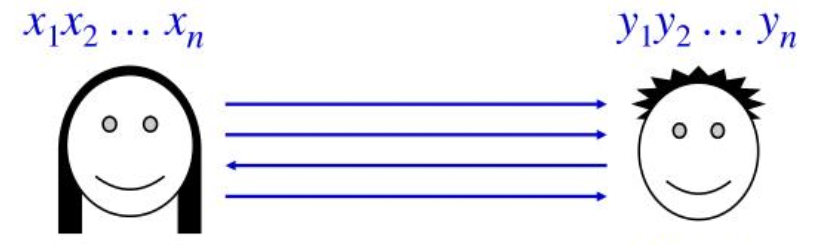
\includegraphics[width=8cm]{1}
    \centering
    \label{fig:001}
    \caption{ماتریس مشخصه یک تابع دلخواه $f: X \times Y \rightarrow \{0, 1\}$ با $X = Y = \{00, 01, 10, 11\}$.}
\end{figure}
به منظور تفهیم‌ بهتر، فرض کنید که $X = Y = \{00, 01, 10, 11\}$ و تابع $f : X \times Y \rightarrow \{0,1\}$ به واسطه ماتریس مشخصه خود در \ref{fig:001} داده شده باشد. یک پروتکل معتبر برای $f$ در شکل \ref{fig:002} نشان داده شده است.
\begin{figure}[h]
    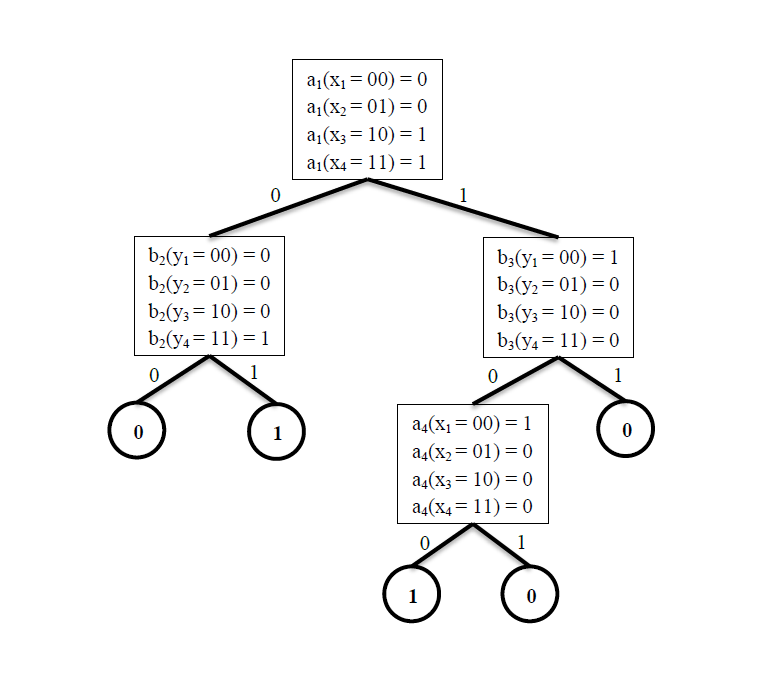
\includegraphics[width=13cm]{2}
    \centering
    \label{fig:002}
    \caption{یک پروتکل صحیح برای مخابره تابع مشخص‌شده در \autoref{fig:001}}
\end{figure}

\subsection{قطعه بندی}
\par
\begin{definition}
تابع  $f : X \times Y \rightarrow \{0,1\} $ را در نظر بگیرید. یک زیر مجموعه $ S \subseteq X \times Y$ $f$- تک‌رنگی\footnote{f-monochromatic} است اگر تابع $f$ روی $S$ ثابت باشد.
\end{definition}

\begin{theorem}
مجموعه ورودی‌های $(x,y) \in X \times Y$ که به یک برگ مشخص از درخت پروتکل ختم می‌شود، یک مستطیل است.
\end{theorem}

نتیجه: هر پروتکل قطعی برای تابع $f$، مجموعه  $X \times Y $ را به مستطیل‌های $f$-تک‌رنگی جدا از هم قطعه‌بندی\footnote{partition} می‌کند. در واقع، حداکثر تعداد مستطیل‌ها $2^{C}$ است که $C$ هزینه ارتباطی پروتکل است (ارتفاع درخت).
\\
بیشینه‌ای که در نتیجه فوق مطرح شده‌است از جایی بر‌می‌آید که درختی با ارتفاع $C$ نمی‌تواند بیشتر از $2^{C}$ برگ داشته باشد.\\
توجه کنید که هر پروتکل، ماتریس مشخصه را به تعدادی مستطیل قطع بندی خواهد کرد ولی هر قطعه‌بندی لزوما معادل یک پروتکل نیست. به عنوان مثال، در شکل \ref{fig:003} نمی‌توان یک پروتکل پیدا کرد چرا که هیچ برشی نیست که بتواند یک زیرماتریس را به دو ماتریس‌ دیگر تبدیل کند  (اولین قدم پروتکل اجرایی نیست).
\begin{figure}[h]
    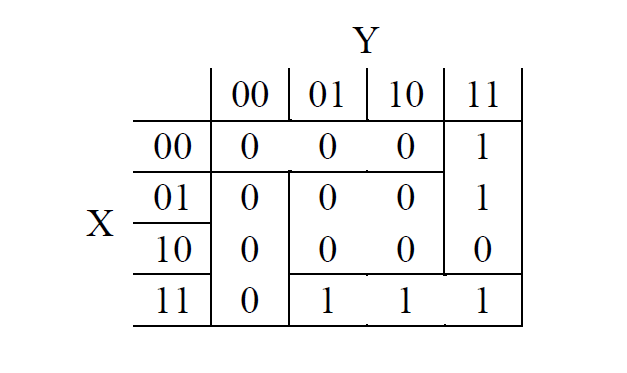
\includegraphics[width=13cm]{3}
    \centering
    \label{fig:003}
    \caption{قطع‌بندی‌ای که نمی‌تواند به یک پروتکل نظیر شود. هیچ برشی در قطعه‌بندی وجود ندارد که با انتخاب آن، ماتریس به دو زیرماتریس تبدیل شود.}
\end{figure}

\subsection{مجموعه گول‌زننده}
به عنوان یک روش برای محاسبه کردن کمینه پیچیدگی ارتباطی یک مساله، می‌توانیم از ابزاری به نام مجموعه گول زننده\footnote{Fooling Set} استفاده کنیم.\\
\begin{definition}
تابع $f : X \times Y \rightarrow \{0,1\}$ داده شده است. یک مجموعه $S \subseteq X \times Y$ را مجموعه گول زننده می‌نامند اگر یک مقدار $z \in \{0,1\}$ وجود داشته باشد به طوری که:
\begin{itemize}
    \item برای هر $(x,y) \in S$ داشته باشیم $f(x,y) = z$.
    \item برای هر دو عضو متفاوت $(x_{1},y_{1})$ و $(x_{2},y_{2})$ در $S$، یا $f(x_{1}, y_{2}) \neq z$ یا $f(x_{2}, y_{1}) \neq z$.
\end{itemize}
\end{definition}
\begin{theorem}
 پیچیدگی ارتباطی تابع $f$ از نامساوی زیر پیروی می‌کند، \\
$D(f) \geq log_{2}|S|$\\
که $S$ هر مجموعه گول زننده‌ای برای $f$ است.
\end{theorem}
\begin{proof}
هیچ دوعضوی از مجموعه گول‌زننده $S$ طبق تعریف نمی‌توانند عضو یک مستطیل در قطعه‌بندی باشند، درنتیجه حداقل به تعداد اعضای $S$، مستطیل $f$-تک‌رنگی داریم. طبق نتیجه قبل، حکم ثابت می‌شود.

\end{proof}
\begin{example}
تابع مساوی را در نظر بگیرید. از قبل می‌دانیم حداکثر تعداد بیت‌هایی که باید برای این مساله مخابره شود $n$ است. حال می‌خواهیم نشان دهیم که این تعداد، حداقل هم هست. تعریف تابع مساوی$EQ_{n} : \{0,1\}^{n} \times \{0,1\}^{n} \rightarrow \{0,1\}$ به صورت زیر خواهد بود
\begin{equation}
    EQ_{n}(x,y) =
    \begin{cases}
        1 & \text{ x=y}\\
        0 & \text{در غیر این صورت}
    \end{cases}
\end{equation}

ماتریس مشخصه این تابع همان ماتریس همانی $2^{n} \times 2^{n}$ است.
\begin{center}
    $\begin{bmatrix}
         1 & 0 & \cdots & 0 \\
         0 & 1 & \cdots & 0 \\
         \vdots & \vdots & \ddots & \vdots \\
         0 & 0 & \cdots & 1
    \end{bmatrix}$
\end{center}
مجموعه گول زننده در این حالت همه مقادیر $1$ تابع $f$ است. چرا که هیچ دوتایی از ورودی‌هایی که خروجی $1$ دارند، در یک مسنطیل نمی‌توانند باشند.  \\
\end{example}
\subsection{کران اندازه مستطیل}
کران اندازه مستطیل\footnote{Rectangle Size Bounds} یک روش دیگر برای اثبات کردن کمینه‌های توابع بولی مورد استفاده در پیچیدگی ارتباطی است. ایده پشت این ماجرا، ثابت کردن آن است که اندازه هر مستطیل کوچک است، در نتیجه باید تعداد زیادی مستطیل برای پوشاندن کل ماتریس مشخصه داشته باشیم. \\
ایده: 
تابع $f : X \times Y \rightarrow \{0,1\}$ داده شده است. روی اعضای $f^{-1}(1)$ یک توزیع احتمال $\mu$ تعریف می‌کنیم به طوری که برای هر مستطیل $R$ شامل مقادیر $1$، $\mu(R) $کوچک باشد. به همین طریق می‌توانیم برای مقادیر $0$ هم این روند را تکرار کنیم. \\
\begin{example}
نشان می‌دهیم که مجموعه گول‌زننده یک مدلی از کران اندازه مستطیل است. فرض کنید که مجموعه گول‌زننده $S$ را داشته باشیم و $|S| = t$. حال $\mu$ را یک توزیع یکنواخت روی اعضای $S$ درنظر بگیرید. در نتیجه
\begin{equation}
    \mu(x,y) =
    \begin{cases}
        $1/t$ & \text{$(x,y) \in S$}\\
        0 & \text{در غیر این صورت}
    \end{cases}
\end{equation}

نشان دادیم که هیچ دو عضوی از مجموعه $S$ نمی‌توانند در یک مستطیل $f$-تک‌رنگی باشند. در نتیجه، برای هر مستطیل $R$ داریم  $\mu(R) \leq 1/t$ و در نهایت باید $\frac{1}{\frac{1}{t}}$ برگ در درخت پروتکل وجود داشته باشد و این گواهی بر این است که  $D(f) \geq \lceil \log_{2} t \rceil$.
\end{example}
\subsection{کمینه رتبه ماتریس \footnote{Matrix Rank}} % TODO : example
\begin{theorem}
تابع $f : X \times Y \rightarrow \{0,1\}$ داده شده است. داریم $D(f) \geq \log_{2}(2\times rank_{F}(M_{f} -1) )$ بر روی هر میدان $F$.
\end{theorem}
\begin{proof}
در قسمت‌های قبل نشان دادیم که پیچیدگی ارتباطی تابع مساوی برابر $n$ است. حال با استفاده از رتبه، این را نشان می‌دهیم: \\
از آنجایی که ماتریس مشخصه تابع مساوی ماتریس همانی $2^{n} \times 2^{n} $ است، و رتبه این ماتریس برابر $2^{n} $ است، طبق قضیه قبل پیچیدگی ارتباطی این مساله $n$ است.
\end{proof}


